\documentclass[preprint,12pt]{elsarticle}

\usepackage{graphicx}
\usepackage{amsmath,amssymb}
\usepackage{booktabs}
\usepackage{multirow}
\usepackage{hyperref}
\usepackage{xcolor}
\usepackage{lineno}
\usepackage{pifont}
\modulolinenumbers[5]

\journal{Expert Systems with Applications}

\begin{document}

\begin{frontmatter}

\title{Does Naive Cross-Validation Inflate Software Energy-Regression Prediction? A Leakage-Aware, Statistically-Gated, Cross-Project Empirical Study}

\author[brac]{Rahat Ahmed Jobu}
\ead{rahatahmed537@gmail.com}

\affiliation[brac]{organization={Department of Computer Science and Engineering, BRAC University},
            city={Dhaka},
            country={Bangladesh}}

\begin{abstract}
Green software engineering has emerged as a response to the growing energy footprint of software systems, yet little work automatically predicts which code commits will regress a project's energy consumption. We construct a cross-project benchmark of 3{,}684 commit transitions across nine open-source projects (seven Java, two Go) by mining diff-based features and combining them with the publicly released EnergyTrackr energy measurements. Regression labels are statistically gated using a Mann--Whitney U test and Cliff's delta effect size on raw per-commit measurement samples. We compare three evaluation protocols and find that naive random-split evaluation overstates predictive performance relative to a leakage-aware leave-one-project-out protocol (pooled out-of-fold ROC-AUC 0.675 vs. 0.506; bootstrap gap 0.168, 95\% CI [0.112, 0.232], $p<0.0001$), a result that is robust to a cluster-level (block-by-project) bootstrap, a false-discovery-rate correction on the labeling procedure, and consistent in direction across Random Forest, XGBoost, and logistic regression. A feature-ablation test attributes roughly 62\% of the gap to one project-identity-correlated feature, with a smaller, still-significant residual gap remaining. A near-duplicate audit and a fold-count-matched redesign together indicate this residual gap reflects genuine cross-project generalization difficulty rather than near-duplicate memorization. Manual verification of a labeled-regression sample, however, found only half correspond to plausible genuine code-efficiency changes, with the remainder attributable to release-metadata commits and test-suite-size growth -- a substantive, openly reported limitation on the benchmark's construct validity. We release the benchmark, labeling protocol, and evaluation code, and argue that project-grouped evaluation, pooled bootstrap significance testing, and label-artifact screening should become standard practice in this emerging area.
\end{abstract}

\begin{keyword}
Green software engineering \sep energy regression \sep data leakage \sep cross-project evaluation \sep explainable machine learning \sep empirical software engineering
\end{keyword}

\end{frontmatter}

\linenumbers

\section{Introduction}
\label{sec:intro}

Information and communication technology is responsible for an estimated 2.1\%--3.9\% of global carbon emissions, and this share is projected to grow as software systems scale~\citep{green2025llmcode}. Green software engineering has consequently emerged as a research area concerned with measuring, understanding, and reducing the energy footprint of software throughout its development lifecycle~\citep{junger2024greencoding,hindle2014greenminer}. A growing body of exploratory work has measured the energy cost of specific libraries, languages, and design choices~\citep{energyrace2025rpython}, and catalogued energy-related code patterns mined from commit histories and issue trackers~\citep{cruz2019catalog}. However, the field remains in an early stage: automatically \emph{predicting}, at commit time, whether a code change will regress a project's energy consumption -- so that it can be flagged before merge, the way a linter or a CI test flags a functional regression -- has received comparatively little attention.

The most directly relevant prior work is EnergyTrackr~\citep{bechet2026energytrackr}, which measured real energy consumption across the commit histories of Java projects using hardware-level (RAPL/\texttt{perf}) instrumentation, and manually identified a small number of statistically significant energy regressions to characterize recurring anti-patterns. EnergyTrackr's contribution is a \emph{detection} pipeline and a qualitative pattern catalog; it does not attempt to turn its measurements into a reusable, cross-project \emph{prediction} benchmark, nor does it examine whether standard machine-learning evaluation protocols -- as commonly used elsewhere in empirical software engineering -- would overstate how well such a predictor generalizes.

This question matters because the broader software-engineering literature has repeatedly found that naive evaluation protocols inflate reported performance when training and test data share hidden structure: near-duplicate instances, temporal ordering violated by random splits, or systematic differences between projects. This failure mode has been documented in cross-project defect prediction~\citep{cpdp2026domainadaptation}, malware detection, and, very recently, in machine-learning-based CI/CD build prediction~\citep{buildpred2026taxonomy}. Kapoor and Narayanan~\cite{kapoor2023leakage} catalog eight general leakage types across 17 scientific fields and find that leakage is associated with substantially inflated, non-reproducible performance claims; similar effects have been shown even in unrelated domains such as connectome-based neuroimaging models~\citep{rosenblatt2024leakage}. No prior work has examined whether this same failure mode affects software energy-regression prediction specifically.

We address this gap with four contributions:
\begin{enumerate}
\item We construct and release a cross-project, cross-language benchmark of 3{,}684 labeled commit transitions across nine open-source projects, built by combining EnergyTrackr's public raw energy measurements with diff-based features mined directly from each project's git history.
\item We introduce a statistically-gated labeling protocol (Mann--Whitney U significance plus a minimum Cliff's delta effect size on raw measurement samples) as a more defensible alternative to a bare percent-change threshold, and we quantify per-project measurement noise to justify the chosen threshold.
\item We conduct a near-duplicate audit of the resulting feature space and show that project-level grouping alone is insufficient to prevent leakage: 48.9\% of transitions share a near-identical diff signature with at least one other transition, motivating a stricter cluster-disjoint evaluation protocol.
\item We quantify, with a statistically rigorous out-of-fold bootstrap procedure rather than a small-sample fold-level comparison, the performance inflation caused by naive evaluation, and show the effect is robust to the choice of regression-labeling threshold.
\end{enumerate}

The remainder of this paper is structured as follows. Section~\ref{sec:related} reviews related work in green software engineering and leakage-aware evaluation. Section~\ref{sec:method} describes the benchmark construction, labeling protocol, and evaluation design. Section~\ref{sec:results} presents the empirical results. Section~\ref{sec:discussion} discusses implications and Section~\ref{sec:threats} discusses threats to validity. Section~\ref{sec:conclusion} concludes and outlines future work.

\section{Related work}
\label{sec:related}

\subsection{Green software engineering}
Measuring software energy consumption has traditionally relied on hardware instrumentation such as Intel RAPL or physical power meters~\citep{hindle2014greenminer}. Building on this measurement infrastructure, exploratory studies have compared the energy cost of programming languages, libraries, and design patterns~\citep{energyrace2025rpython}, and mined GitHub commits, issues, and pull requests that mention energy or battery concerns to build catalogs of energy-improving code patterns~\citep{cruz2019catalog}. Junger et al.~\cite{junger2024greencoding} synthesize this line of work into recommendations for industry and education. Most recently, Bechet et al.~\cite{bechet2026energytrackr} introduced EnergyTrackr, which detects energy regressions across a project's commit history using repeated hardware measurements and statistical outlier filtering, and manually characterizes recurring anti-patterns (e.g., missing early exits, costly dependency upgrades) from the flagged commits. Our work is complementary: whereas EnergyTrackr is a per-project \emph{detection} pipeline evaluated via manual pattern analysis, we reuse its public measurements to build a \emph{predictive}, cross-project benchmark and focus specifically on whether standard evaluation protocols for such a predictor are trustworthy.

\subsection{Leakage-aware evaluation in software engineering prediction tasks}
Data leakage -- where information not legitimately available at prediction time inflates apparent model performance -- is a well-documented problem across empirical machine learning. Kapoor and Narayanan~\cite{kapoor2023leakage} identify eight leakage types (including duplicate data points and non-independence between train and test sets) across a meta-review of 329 papers spanning 17 scientific fields, and find leakage is systematically associated with inflated, non-reproducible results. Within software engineering specifically, cross-project defect prediction has confronted this problem for over a decade: near-duplicate or oversampled instances crossing the train/test boundary are known to inflate reported generalization~\citep{cpdp2026domainadaptation}. Very recently, a taxonomy study~\cite{buildpred2026taxonomy} released an open-source leakage-detection toolkit for machine-learning-based CI/CD build prediction, explicitly designed to generalize to ``defect prediction, test selection, and code review prioritization'' -- but not to energy-regression prediction. Table~\ref{tab:related} positions the present study against this literature along the dimensions most relevant to our contribution.

\begin{table}[htbp]
\centering
\caption{Positioning of this study against the most closely related prior work.}
\label{tab:related}
\resizebox{\textwidth}{!}{%
\begin{tabular}{@{}lccccc@{}}
\toprule
Study & Task & Cross-project & Leakage-aware eval. & Statistically-gated labels & Explainability \\
\midrule
EnergyTrackr~\citep{bechet2026energytrackr} & Energy regression \emph{detection} & \ding{55}\ (single-project) & \ding{55} & \checkmark\ (IQR outlier filter) & \ding{55} \\
Catalog of Energy Patterns~\citep{cruz2019catalog} & Pattern mining (mentions) & \checkmark & n/a (not predictive) & \ding{55} & \ding{55} \\
CPDP leakage study~\citep{cpdp2026domainadaptation} & Defect \emph{prediction} & \checkmark & \checkmark\ (dedup) & \ding{55} & \ding{55} \\
Build-prediction leakage taxonomy~\citep{buildpred2026taxonomy} & Build outcome \emph{prediction} & \checkmark & \checkmark\ (temporal) & \ding{55} & \ding{55} \\
\textbf{This work} & Energy regression \emph{prediction} & \checkmark\ (Java + Go) & \checkmark\ (project + cluster-disjoint) & \checkmark\ (Mann--Whitney + effect size) & \checkmark\ (SHAP) \\
\bottomrule
\end{tabular}%
}
\end{table}

\subsection{Statistical rigor in performance comparison}
Beyond leakage, small-sample significance testing is itself a common source of overclaiming: comparing only a handful of cross-validation fold means, as is common practice, has limited statistical power to detect real differences. We are not aware of prior software-energy work that addresses this specifically; we adopt an out-of-fold prediction bootstrap, standard in the broader machine-learning evaluation literature but, to our knowledge, not previously applied to this comparison in the green software engineering literature.

\section{Methodology}
\label{sec:method}

Figure~\ref{fig:pipeline} summarizes the end-to-end pipeline, described in detail below.

\begin{figure}[htbp]
\centering
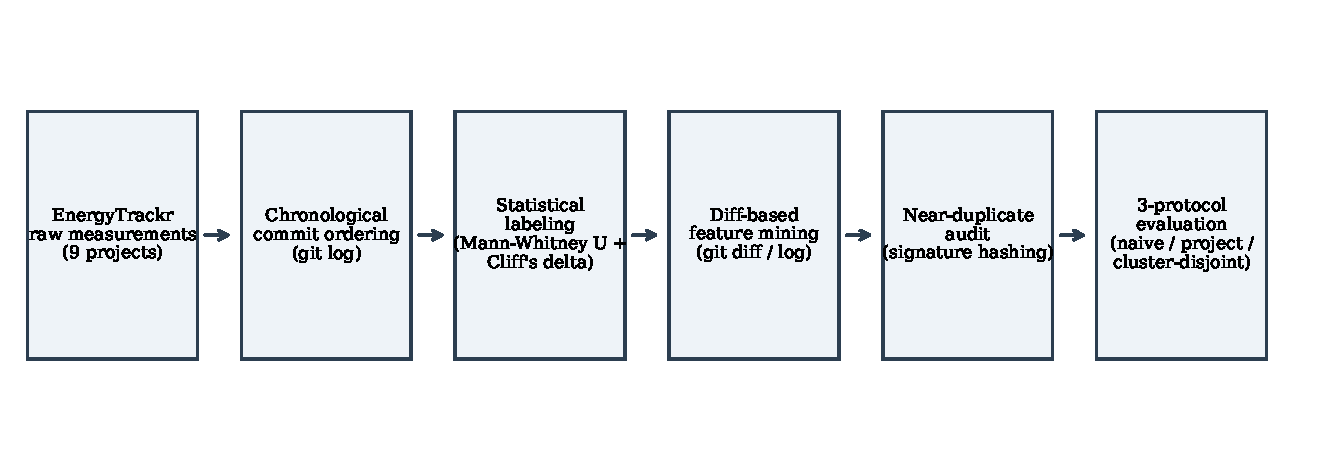
\includegraphics[width=\textwidth]{figures/fig1_pipeline.pdf}
\caption{Overview of the benchmark construction and evaluation pipeline.}
\label{fig:pipeline}
\end{figure}

\subsection{Data source}
\label{sec:datasource}
We build on the public data release accompanying EnergyTrackr~\citep{bechet2026energytrackr}, which contains raw per-commit energy measurements (in joules) collected via \texttt{perf}/RAPL on a fixed hardware profile, with approximately 15 repeated measurement runs per commit. Of the projects in the release, nine have complete, usable measurement files: seven Java projects (\texttt{docx4j}, \texttt{fastexcel}, \texttt{flexy-pool}, \texttt{jacoco}, \texttt{jsoup}, \texttt{signalfx-java}, \texttt{super-csv}) and two Go projects (\texttt{fiber}, \texttt{nscache}). We do not attempt to remeasure energy consumption ourselves: hardware power-domain instrumentation (RAPL) requires bare-metal access unavailable in commodity cloud compute environments, so building on an existing, independently collected measurement release is the only reproducible option for this study without dedicated hardware.

\subsection{Statistically-gated regression labeling}
\label{sec:labeling}
For each project, we recover the true chronological order of measured commits from the project's git history and consider every consecutive pair of \emph{measured} commits as a transition. A naive labeling approach -- used implicitly by percent-change thresholds elsewhere in the literature, and matching EnergyTrackr's own default configuration -- labels a transition a ``regression'' if the median energy increases by more than 20\%. This point-estimate approach does not account for measurement noise: with only $\sim$15 samples per commit, a 20\% shift in the median could in principle reflect noise rather than a real effect.

We therefore compute, for every transition, a Mann--Whitney U test between the previous and current commit's raw measurement samples, and Cliff's delta effect size $\delta = \frac{|\{(x,y): x>y\}| - |\{(x,y): x<y\}|}{n_1 n_2}$. A transition is labeled a statistically-gated regression only if it exceeds the 20\% median threshold \emph{and} the difference is significant ($p<0.05$) \emph{and} the effect size is at least medium ($|\delta|>0.33$, following the conventional categorization of~\cite{romano2006exploring}). We report both the naive and statistically-gated label counts; empirically, in our dataset the two agree almost exactly (Section~\ref{sec:results}), because median per-commit measurement noise (coefficient of variation) never exceeds 3.4\% across the nine projects -- well below the 20\% regression threshold -- providing direct empirical evidence that the threshold is not merely detecting noise.

We note that running 3{,}684 independent significance tests at $p<0.05$ without correction would, under a global null hypothesis of no true regressions, yield approximately 184 false positives by chance alone -- far more than the 52 transitions our conjunctive criterion ultimately labels as regressions. The three-way conjunction (percent-change threshold \emph{and} significance \emph{and} medium-or-larger effect size) is considerably more conservative than a raw $p<0.05$ cutoff and is the primary defense against this risk. We additionally verified this directly with a Benjamini--Hochberg false-discovery-rate correction across all 3{,}684 tests (Section~\ref{sec:bhresults}): all 52 gated regressions remain significant after correction, confirming the conjunctive criterion's implicit protection empirically rather than leaving it as an untested assumption.

\subsection{Feature engineering}
For each labeled transition we mine diff-based features directly from the project's cloned git repository: lines added/deleted, net churn, files changed, the number of intervening (unmeasured) commits, commit-message length, and five keyword indicators (performance, fix, test, refactor, dependency) matched against intervening commit messages. Skewed count features (churn, files changed, commits between) are log-transformed; we additionally derive an add/delete ratio, churn-per-file, and a log-transformed previous-commit energy baseline.

\subsection{Near-duplicate audit}
\label{sec:dupaudit}
Prior cross-project prediction studies typically prevent leakage only by grouping folds at the project level. We additionally audit the feature space for \emph{within}-project near-duplicates: many commits are trivial, repetitive changes (e.g., single-line dependency-version bumps) that produce near-identical diff signatures. We hash each transition on a coarse signature (lines added/deleted, files changed, and the five keyword indicators) and treat transitions sharing a signature within the same project as a near-duplicate cluster. This audit (Section~\ref{sec:results}) reveals that project grouping alone does not fully address the leakage risk in this task.

\subsection{Evaluation protocols}
We compare three evaluation protocols for a Random Forest classifier (balanced-subsample class weighting, max depth 5, minimum leaf size 3, chosen to control overfitting given the severe class imbalance; 400 trees during all cross-validation evaluation to limit computational cost across the many folds and bootstrap iterations required, and 500 trees for the single final model fit to the complete dataset for the explainability analysis in Section~\ref{sec:results}). All model fitting, data splitting, and bootstrap resampling use a fixed random seed (42) throughout, and the full implementation is included in the released replication package (see Data Availability). The three protocols compared are:
\begin{itemize}
\item \textbf{Naive}: 5-fold stratified cross-validation with random shuffling, ignoring project and duplicate structure -- the protocol implicitly assumed by a bare train/test split.
\item \textbf{Project-grouped}: leave-one-project-out cross-validation (\texttt{GroupKFold} by project), simulating the realistic deployment scenario of a new project with no prior energy-labeled history.
\item \textbf{Cluster-disjoint}: 5-fold \texttt{GroupKFold} grouped by project \emph{and} near-duplicate signature jointly, a stricter protocol that also prevents near-identical trivial commits from splitting across folds even within held-out projects.
\end{itemize}
For each protocol we report ROC-AUC and PR-AUC (average precision), alongside a \texttt{DummyClassifier} stratified-random baseline as a chance-level sanity check, and a training-free heuristic baseline: ranking transitions by raw net code churn, adapting the long-established code-churn-based defect-proneness heuristic of Nagappan and Ball~\cite{nagappan2005churn} to this task. Because this heuristic requires no fitting at all, it cannot leak by construction and needs no protocol-specific training, making it a useful reference point for how much of the fitted models' apparent performance reflects genuine learned signal versus what a simple, well-motivated rule already captures. We are not aware of any published machine-learning predictor for this exact task (energy-regression prediction from commit diffs) to compare against; EnergyTrackr~\citep{bechet2026energytrackr} performs detection via statistical outlier filtering on measured energy rather than prediction from code features, and is therefore not a comparable predictive baseline. Consequently, our comparison is between evaluation protocols and against this training-free heuristic, not between our method and a competing predictive approach -- we regard establishing this reference point, imperfect as it is, as part of this paper's contribution, and we explicitly do not claim our Random Forest, XGBoost, or logistic regression results represent a validated advance over prior predictive work, since no such prior work exists to be advanced upon. To test whether the naive-vs-project-grouped performance gap is statistically real rather than an artifact of comparing a handful of fold-level numbers (which has limited statistical power at $k=5$--$9$ folds), we additionally collect out-of-fold predictions for every transition under each protocol and run a stratified bootstrap (2{,}000 resamples) over the pooled predictions to obtain a confidence interval and two-sided p-value on the AUC gap. Finally, we sweep the regression-labeling threshold across $\{10\%, 15\%, 20\%, 25\%, 30\%\}$ to test whether the naive-vs-grouped gap is an artifact of the single 20\% default inherited from EnergyTrackr's configuration.

\subsection{Robustness and diagnostic checks}
\label{sec:robustness}
Following an internal self-audit of an earlier draft of this work, we conducted six additional checks to interrogate rather than merely restate our headline finding: (1) a feature-ablation test of whether the previous-commit energy baseline drives the naive-protocol gap; (2) a comparison across three algorithm families rather than Random Forest alone; (3) a comparison against a training-free code-churn heuristic baseline, since no prior predictive method for this task exists to compare against; (4) a Benjamini--Hochberg false-discovery-rate correction across all labeling significance tests; (5) a cluster-level (block-by-project) bootstrap as a more conservative alternative to the row-level bootstrap above, since row-level resampling treats out-of-fold predictions as independent even though predictions from the same held-out fold share a common trained model; and (6) a fold-count-matched redesign of the cluster-disjoint protocol that removes the confound identified in Section~\ref{sec:discussion}, together with a manual inspection of a sample of labeled regressions. Results are reported in Section~\ref{sec:results}.

\section{Results}
\label{sec:results}

\subsection{Dataset composition}
The final benchmark comprises 3{,}684 labeled commit transitions (3{,}015 Java, 669 Go) across nine projects, with 52 transitions (1.41\%) meeting the statistically-gated regression criterion. Table~\ref{tab:breakdown} and Figure~\ref{fig:breakdown} show the per-project composition. Regression rates vary substantially across projects (0\%--7.8\%), and two projects (\texttt{flexy-pool}, \texttt{signalfx-java}) and one Go project (\texttt{fiber}) contain zero statistically-gated regressions, which we return to in Section~\ref{sec:threats}.

\begin{table}[htbp]
\centering
\caption{Per-project dataset composition. ``Naive'' and ``Gated'' report regression counts under the bare-threshold and statistically-gated labeling protocols, respectively (Section~\ref{sec:labeling}).}
\label{tab:breakdown}
\begin{tabular}{@{}llrrrr@{}}
\toprule
Language & Project & Transitions & Naive regressions & Gated regressions & Positive rate \\
\midrule
Go   & fiber         & 538  & 0  & 0  & 0.000 \\
Go   & nscache       & 131  & 3  & 3  & 0.023 \\
Java & docx4j        & 90   & 7  & 7  & 0.078 \\
Java & fastexcel     & 637  & 15 & 15 & 0.024 \\
Java & flexy-pool    & 10   & 0  & 0  & 0.000 \\
Java & jacoco        & 199  & 5  & 5  & 0.025 \\
Java & jsoup         & 1985 & 19 & 19 & 0.010 \\
Java & signalfx-java & 14   & 0  & 0  & 0.000 \\
Java & super-csv     & 80   & 3  & 3  & 0.038 \\
\midrule
\multicolumn{2}{l}{\textbf{Total}} & \textbf{3684} & \textbf{52} & \textbf{52} & \textbf{0.014} \\
\bottomrule
\end{tabular}
\end{table}

\begin{figure}[htbp]
\centering
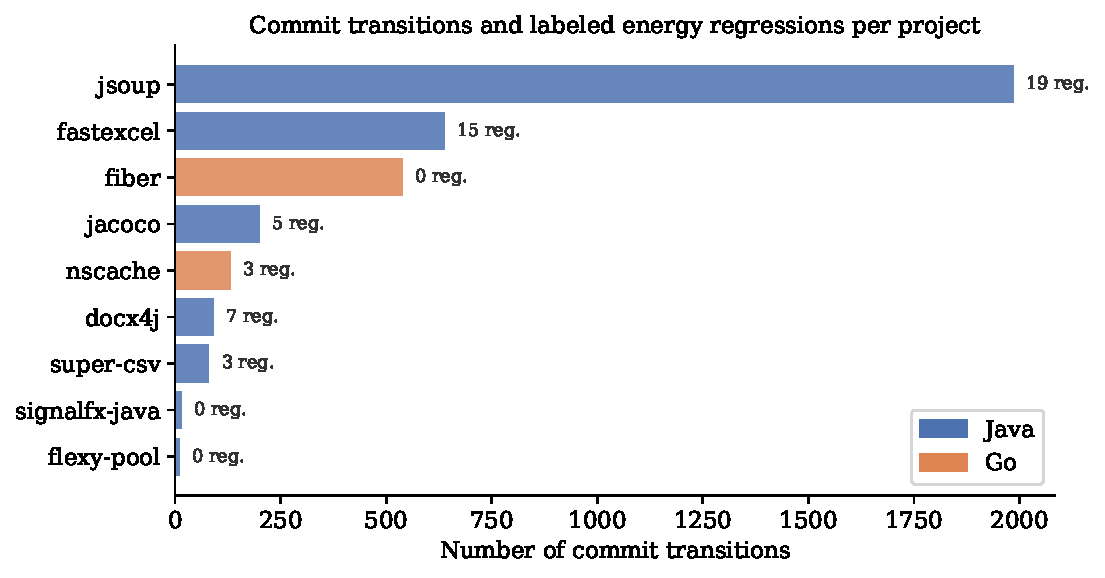
\includegraphics[width=0.8\textwidth]{figures/fig2_breakdown.pdf}
\caption{Commit transitions and labeled energy regressions per project.}
\label{fig:breakdown}
\end{figure}

Median per-commit measurement coefficient of variation ranged from 0.2\% (\texttt{fiber}) to 3.4\% (\texttt{flexy-pool}) across projects, confirming that the 20\% regression threshold sits well above the measurement noise floor for every project in the benchmark, and explaining why the naive and statistically-gated labels coincide exactly in our data (Table~\ref{tab:breakdown}).

\subsection{Near-duplicate audit}
The near-duplicate audit (Section~\ref{sec:dupaudit}) identified 280 near-duplicate signature groups, involving 1{,}801 of 3{,}684 transitions (48.9\%) -- see Figure~\ref{fig:dupaudit}. This confirms that project-level grouping alone leaves substantial within-project redundancy unaddressed, motivating the cluster-disjoint protocol introduced in Section~\ref{sec:method}.

\begin{figure}[htbp]
\centering
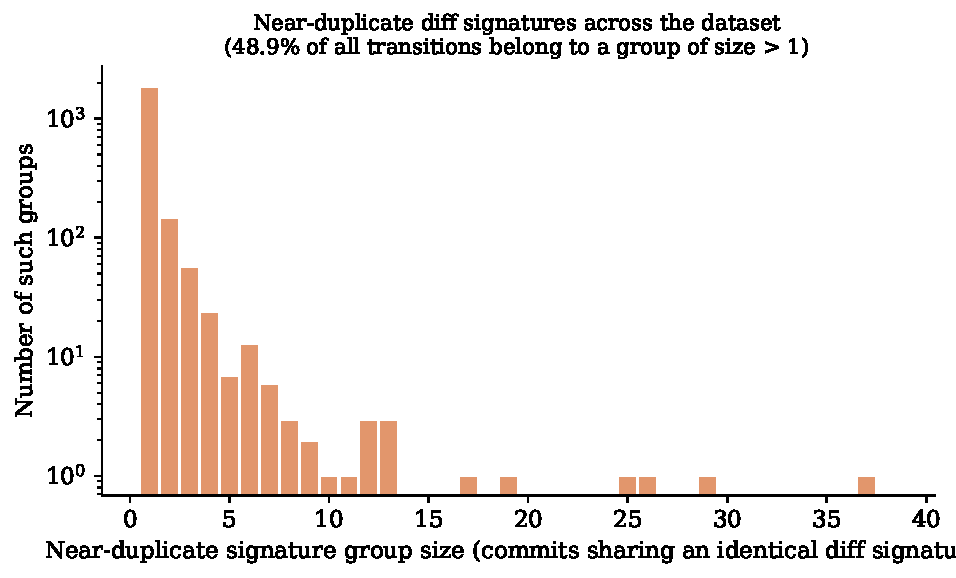
\includegraphics[width=0.7\textwidth]{figures/fig7_near_duplicate_audit.pdf}
\caption{Distribution of near-duplicate diff-signature group sizes (log-scaled y-axis). Nearly half of all transitions belong to a group of size greater than one.}
\label{fig:dupaudit}
\end{figure}

\subsection{Naive vs. leakage-aware evaluation}
Table~\ref{tab:protocols} and Figure~\ref{fig:protocols} report ROC-AUC and PR-AUC under all three protocols. The naive protocol reports a ROC-AUC of 0.681 ($\pm$0.087), while the project-grouped protocol drops to 0.545 ($\pm$0.230); the cluster-disjoint protocol falls between the two (0.659 $\pm$ 0.073). \emph{We flag immediately that this particular cluster-disjoint number is later shown (Section~\ref{sec:redesign}) to be confounded by a fold-count difference rather than a clean measurement of near-duplicate effects; a corrected, fold-count-matched version (0.488) is reported in Section~\ref{sec:redesign} and is the number we rely on for our conclusions about near-duplicate memorization. We retain this original result here for transparency about what our initial protocol design actually measured.} All three protocols exceed their respective dummy-classifier baselines ($\approx$0.50) on mean ROC-AUC, but for the project-grouped protocol this margin (0.545 vs.\ 0.504) is small relative to the fold-level standard deviation (0.230), so it should not be read as a confirmed, statistically distinguishable separation from chance on its own; the pooled, bootstrapped comparison in Section~\ref{sec:results} is the appropriate basis for that claim, and we did not additionally bootstrap the model-vs-dummy comparison specifically within the project-grouped protocol.

We note an important discrepancy between the two metrics: PR-AUC under the naive protocol (0.051) is \emph{lower} than under the project-grouped protocol (0.101), the opposite direction from the ROC-AUC comparison. We do not consider this a refutation of the ROC-AUC finding -- PR-AUC is highly sensitive to the precision achieved on the very small number of positives in each fold, and the project-grouped PR-AUC's standard deviation (0.147) is larger than its own mean, indicating the estimate is dominated by one or two folds with a small number of correct top-ranked predictions rather than a stable, generalizable precision advantage. We report this discrepancy openly rather than presenting only the metric that supports our narrative, and we treat the ROC-AUC finding -- corroborated by the pooled out-of-fold bootstrap in Section~\ref{sec:results}, which is far more stable than either raw per-fold metric -- as the more reliable basis for our central claim.

\begin{table}[htbp]
\centering
\caption{Evaluation results across the three protocols (mean $\pm$ std. across folds) and the corresponding dummy-classifier baseline.}
\label{tab:protocols}
\begin{tabular}{@{}lccc@{}}
\toprule
Protocol & ROC-AUC & PR-AUC (Avg. Precision) & Dummy baseline (ROC-AUC) \\
\midrule
Naive (random 5-fold)          & 0.681 $\pm$ 0.087 & 0.051 $\pm$ 0.018 & 0.502 \\
Project-grouped (leave-one-out) & 0.545 $\pm$ 0.230 & 0.101 $\pm$ 0.147 & 0.504 \\
Cluster-disjoint (5-fold)       & 0.659 $\pm$ 0.073 & 0.058 $\pm$ 0.031 & 0.493 \\
\bottomrule
\end{tabular}
\end{table}

\begin{figure}[htbp]
\centering
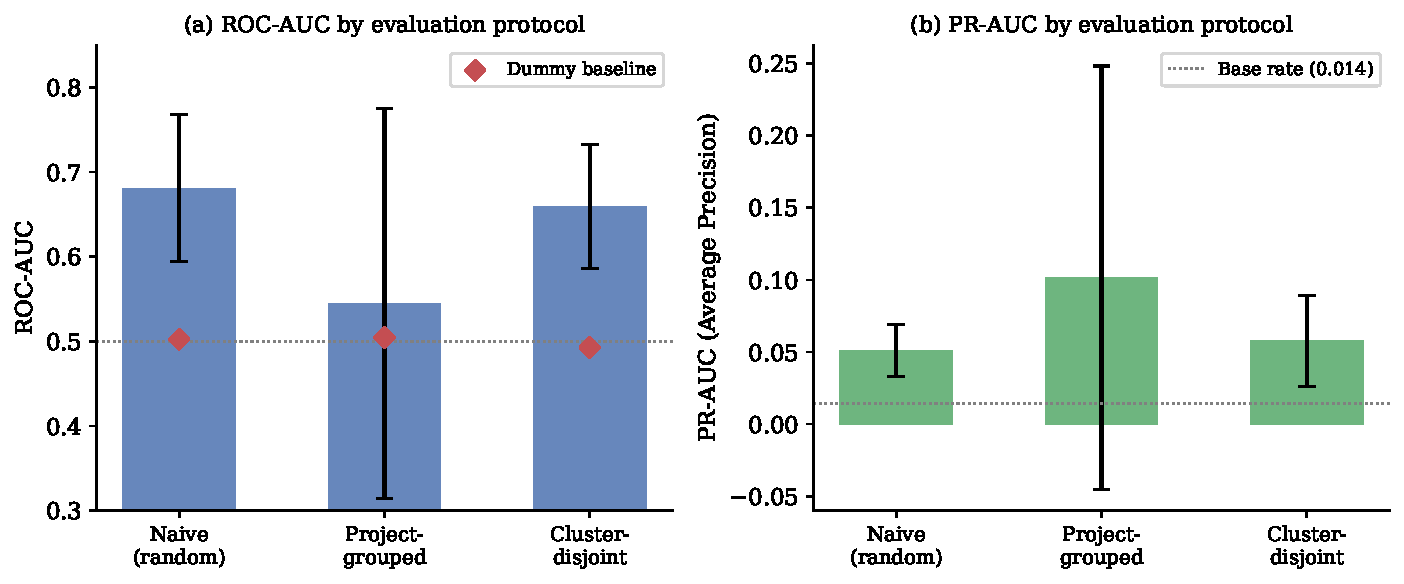
\includegraphics[width=\textwidth]{figures/fig3_protocol_comparison.pdf}
\caption{ROC-AUC (a) and PR-AUC (b) across the three evaluation protocols, with dummy-classifier baselines shown as diamonds/dotted lines.}
\label{fig:protocols}
\end{figure}

The raw fold-level standard deviations in Table~\ref{tab:protocols} are themselves informative: the project-grouped protocol's ROC-AUC standard deviation (0.230) is roughly $2.6\times$ larger than the naive protocol's (0.087), because several held-out projects (Table~\ref{tab:breakdown}) contain very few or zero positive labels, making per-project fold estimates individually unstable. This motivates our use of pooled out-of-fold bootstrapping, rather than the raw per-fold numbers in Table~\ref{tab:protocols}, for statistical inference on the naive-vs-grouped gap.

\subsection{Statistical significance of the leakage gap}
Pooling out-of-fold predictions across all 3{,}684 transitions, naive evaluation achieves ROC-AUC 0.675 versus 0.506 for project-grouped evaluation. A stratified bootstrap over 2{,}000 resamples of these pooled predictions (Figure~\ref{fig:bootstrap}) yields a mean gap of 0.168 with a 95\% confidence interval of [0.112, 0.232] and a two-sided $p<0.0001$, indicating the naive protocol's apparent advantage is not a small-sample artifact. We emphasize that an initial attempt to test significance using only the five raw project-grouped fold means (as is common practice) yielded a non-significant permutation-test result ($p=0.32$) purely due to insufficient statistical power at that sample size -- underscoring that the pooled out-of-fold bootstrap, not a fold-mean comparison, is the appropriate test for this kind of claim.

\begin{figure}[htbp]
\centering
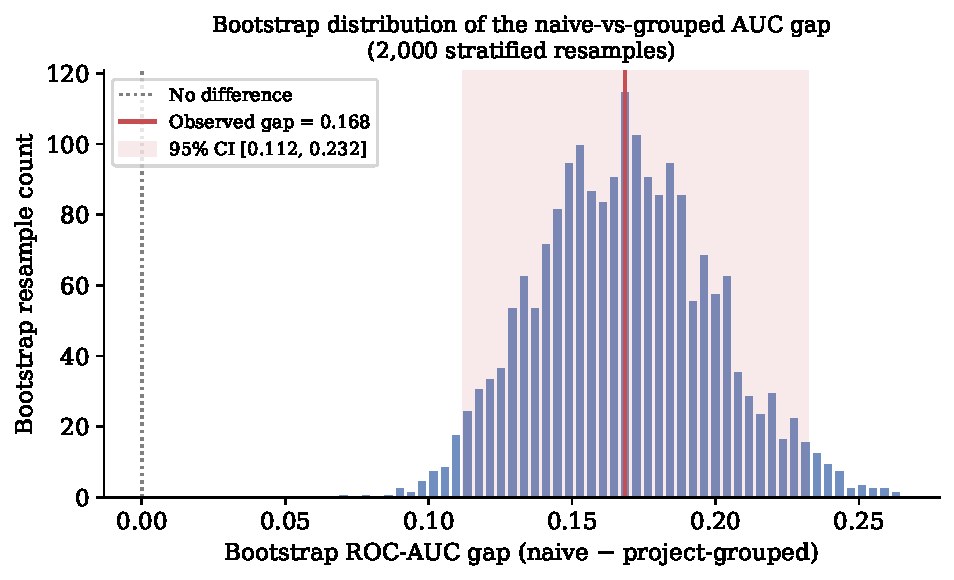
\includegraphics[width=0.7\textwidth]{figures/fig4_bootstrap_gap.pdf}
\caption{Bootstrap distribution (2{,}000 resamples) of the naive-vs-project-grouped ROC-AUC gap. The 95\% confidence interval excludes zero.}
\label{fig:bootstrap}
\end{figure}

\subsection{Threshold sensitivity}
Table~\ref{tab:threshold} and Figure~\ref{fig:threshold} report the naive and project-grouped ROC-AUC across five regression-labeling thresholds. The direction of the gap (naive $>$ grouped) holds at every threshold tested, and the gap is substantially larger at 20--30\% (0.124--0.145) than at 10\% (0.042). The pattern is not strictly monotonic, however: the gap is smallest of all at 15\% (0.023), dipping below the 10\% value before rising sharply from 20\% onward. We do not have a confirmed explanation for this non-monotonicity and note it rather than smoothing over it; it may reflect the small, discrete changes in which specific commits enter or leave the positive class as the threshold moves (Table~\ref{tab:threshold}, \# Positive column drops from 67 to 61 between 10\% and 15\%), which can shift fold composition unpredictably given how few positives exist in total. We caution that each threshold's estimate in Table~\ref{tab:threshold} is a single-run point estimate without a bootstrap confidence interval (unlike the primary 20\%-threshold result in Section~\ref{sec:results}), and should be read as indicative of the gap's persistence in direction rather than as a precisely quantified trend.

\begin{table}[htbp]
\centering
\caption{Threshold sensitivity: naive vs.\ project-grouped ROC-AUC across five regression-labeling thresholds.}
\label{tab:threshold}
\begin{tabular}{@{}crccc@{}}
\toprule
Threshold & \# Positive & Naive ROC-AUC & Grouped ROC-AUC & Gap \\
\midrule
10\% & 67 & 0.691 & 0.649 & 0.042 \\
15\% & 61 & 0.651 & 0.629 & 0.023 \\
20\% & 52 & 0.677 & 0.553 & 0.124 \\
25\% & 50 & 0.683 & 0.540 & 0.143 \\
30\% & 49 & 0.679 & 0.534 & 0.145 \\
\bottomrule
\end{tabular}
\end{table}

\begin{figure}[htbp]
\centering
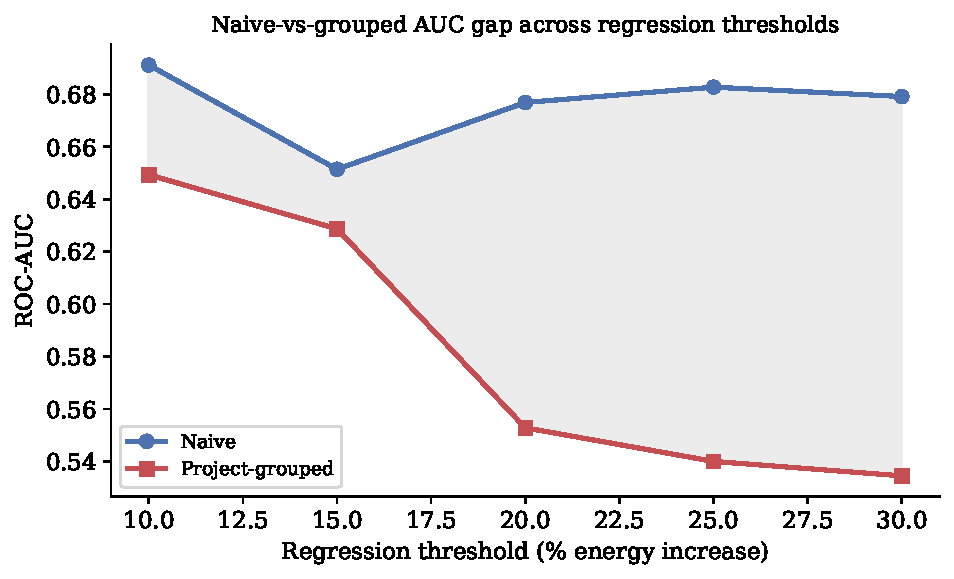
\includegraphics[width=0.7\textwidth]{figures/fig5_threshold_sensitivity.pdf}
\caption{Naive vs.\ project-grouped ROC-AUC across regression thresholds from 10\% to 30\%.}
\label{fig:threshold}
\end{figure}

\subsection{Isolating the source of the gap: feature ablation}
\label{sec:ablation}
Section~\ref{sec:discussion} (in an earlier draft) flagged, as an untested hypothesis, that the previous-commit energy baseline feature (\texttt{log\_prev\_energy}) might allow the naive protocol to partly exploit project identity rather than genuine diff-level signal, since absolute energy readings differ by roughly an order of magnitude across projects. We tested this directly by retraining under both protocols with this feature removed. The result is decisive but partial: removing \texttt{log\_prev\_energy} shrinks the pooled naive ROC-AUC from 0.675 to 0.580 and the gap from 0.168 to 0.064 (95\% CI [0.008, 0.122], $p=0.028$) -- a $\sim$62\% reduction in the gap's magnitude, confirming the hypothesis was substantially correct, while the gap remains statistically significant even without this feature, indicating a genuine, smaller residual leakage effect beyond project-identity encoding. We report both numbers in Table~\ref{tab:ablation} and recommend that future work on this task either exclude absolute energy-scale features or explicitly normalize them within project before use.

\begin{table}[htbp]
\centering
\caption{Feature-ablation results: naive-vs-project-grouped ROC-AUC gap with and without the previous-commit energy baseline feature.}
\label{tab:ablation}
\begin{tabular}{@{}lccc@{}}
\toprule
Feature set & Naive ROC-AUC & Grouped ROC-AUC & Bootstrap gap (95\% CI) \\
\midrule
With \texttt{log\_prev\_energy} (full)   & 0.675 & 0.506 & 0.168 [0.112, 0.232] \\
Without \texttt{log\_prev\_energy}       & 0.580 & 0.517 & 0.064 [0.008, 0.122] \\
\bottomrule
\end{tabular}
\end{table}

\subsection{Robustness across algorithms}
\label{sec:algcompare}
We repeated the naive-vs-project-grouped comparison for two additional algorithm families -- XGBoost (300 trees, max depth 4, learning rate 0.05, \texttt{scale\_pos\_weight} set to the negative/positive class ratio) and logistic regression (L2-regularized, balanced class weighting, up to 2{,}000 solver iterations) -- alongside Random Forest, using the full feature set and the same fixed random seed (42). Neither additional algorithm's hyperparameters were tuned via search; they use scikit-learn/XGBoost defaults adjusted only for class imbalance, consistent with our exploratory, diagnostic purpose here rather than a claim of optimized performance. Table~\ref{tab:algorithms} reports both the raw per-fold means (as conventionally reported) and the pooled out-of-fold bootstrap gap (our recommended method, Section~\ref{sec:method}). The raw fold-mean comparison is unstable: logistic regression's project-grouped fold mean (0.768) appears \emph{higher} than its naive fold mean (0.700), the opposite direction from Random Forest and XGBoost, which would superficially suggest the leakage effect is model-specific or even reverses for linear models. However, once evaluated via the pooled out-of-fold bootstrap, the direction is consistent across all three algorithms (naive $>$ grouped, all $p<0.05$), and the apparent reversal for logistic regression's fold-mean was an artifact of averaging only 9 unweighted per-project fold estimates, several of which carry very few positives. This is a direct, concrete illustration of exactly the fold-averaging instability problem motivating our use of pooled out-of-fold bootstrapping (Section~\ref{sec:method}): naive fold-averaging is not a reliable basis for comparing evaluation protocols at this sample size, and this finding strengthens rather than weakens our methodological argument for pooled bootstrap evaluation.

\begin{table}[htbp]
\centering
\caption{Algorithm comparison. ``Fold-mean'' columns are simple averages across per-fold AUCs (the conventional but, per Section~\ref{sec:algcompare}, unreliable method at this sample size); ``Pooled'' columns use out-of-fold predictions (our recommended method).}
\label{tab:algorithms}
\resizebox{\textwidth}{!}{%
\begin{tabular}{@{}lccccc@{}}
\toprule
Algorithm & Naive (fold-mean) & Grouped (fold-mean) & Naive (pooled) & Grouped (pooled) & Bootstrap gap ($p$-value) \\
\midrule
Random Forest        & 0.681 & 0.545 & 0.675 & 0.506 & 0.168 ($p<0.0001$) \\
XGBoost               & 0.678 & 0.416 & 0.674 & 0.444 & 0.231 ($p<0.0001$) \\
Logistic Regression   & 0.700 & 0.768 & 0.703 & 0.622 & 0.080 ($p=0.020$) \\
\bottomrule
\end{tabular}%
}
\end{table}

\subsection{Comparison against a training-free heuristic baseline}
\label{sec:heuristic}
Table~\ref{tab:heuristic} compares the fitted models against the churn-magnitude heuristic described in Section~\ref{sec:method}. Because the heuristic requires no fitting, its naive and project-grouped scores are computed by simply ranking the same fixed churn values within each protocol's held-out fold -- there is no possibility of it overfitting or leaking training-set structure, so any protocol-dependent difference in its own score reflects only the composition of each fold's positives and negatives, not model behavior.

\begin{table}[htbp]
\centering
\caption{Fitted models vs. the training-free churn-magnitude heuristic baseline (Section~\ref{sec:heuristic}), pooled out-of-fold ROC-AUC.}
\label{tab:heuristic}
\begin{tabular}{@{}lccc@{}}
\toprule
Model & Naive ROC-AUC & Project-grouped ROC-AUC & Naive$-$grouped gap \\
\midrule
Churn-magnitude heuristic (no training) & 0.642 & 0.616 & 0.026 \\
Random Forest        & 0.681 & 0.545 & 0.136 \\
XGBoost               & 0.678 & 0.416 & 0.262 \\
Logistic Regression   & 0.700 & 0.768 & $-0.068$ \\
\bottomrule
\end{tabular}
\end{table}

Two findings are worth stating plainly rather than downplaying. First, the heuristic's own naive-vs-grouped gap (0.026) is far smaller than Random Forest's (0.136) or XGBoost's (0.262), consistent with our broader argument that naive-protocol inflation is substantially a property of what fitted models learn to exploit (Section~\ref{sec:ablation}), not an inherent property of the underlying task. Second, and more humbling, the untrained heuristic's project-grouped ROC-AUC (0.616) exceeds both Random Forest (0.545) and XGBoost (0.416) under the realistic evaluation protocol, and is only modestly below logistic regression's raw fold-mean (0.768, though recall from Section~\ref{sec:algcompare} that this specific number is unstable and the more reliable pooled logistic-regression estimate is 0.622, essentially matching the heuristic). This indicates that, at the current feature-engineering maturity of this task, a simple, well-established, training-free rule from the defect-prediction literature~\citep{nagappan2005churn} is a genuinely competitive predictor -- the added complexity of tree-based ensembles does not yet demonstrate a clear, reliable advantage over it under realistic cross-project deployment conditions. We report this honestly as a finding that tempers any impression that machine learning is straightforwardly necessary or beneficial for this task as currently formulated, rather than omitting or minimizing it.
\subsection{Multiple-comparisons correction}
\label{sec:bhresults}
Applying a Benjamini--Hochberg false-discovery-rate correction across all 3{,}684 labeling significance tests (Section~\ref{sec:labeling}) reduces the raw-significant count from 533 ($p<0.05$ uncorrected) to 289 ($p_{\mathrm{adj}}<0.05$). Critically, all 52 of the original statistically-gated regressions remain significant after correction -- the conjunctive labeling criterion (percent-change threshold \emph{and} significance \emph{and} medium-or-larger effect size) already selects transitions with p-values far below the levels affected by the correction. This directly resolves the multiple-comparisons concern raised in Section~\ref{sec:labeling}: the risk was real to check, but empirically did not affect this dataset's labels.

\subsection{Cluster-aware bootstrap}
\label{sec:clusterboot}
As a more conservative alternative to the row-level bootstrap in Section~\ref{sec:results}, which implicitly treats out-of-fold predictions as independent despite within-fold correlation from a shared trained model, we additionally ran a block bootstrap that resamples whole \emph{projects} (with replacement) rather than individual rows. This gives a mean gap of 0.158 with a wider, more honest 95\% CI of [0.062, 0.280] ($p=0.007$) -- similar in magnitude to the row-level estimate but with appropriately larger uncertainty. The finding survives this more conservative test. We note, however, that with only 9 projects to resample from, the space of achievable bootstrap resamples is combinatorially limited (at most $\binom{17}{9}=24{,}310$ distinct multiset compositions when resampling 9 draws with replacement from 9 items), so this interval's coverage properties are necessarily approximate rather than asymptotically guaranteed; we report it as a useful robustness check and directional confirmation, not as a fully calibrated alternative to the row-level estimate.

\subsection{Redesigned cluster-disjoint protocol}
\label{sec:redesign}
To resolve the fold-count confound identified in Section~\ref{sec:discussion}, we reran the cluster-disjoint comparison holding fold count fixed at 9 (matching the project-grouped protocol exactly) and instead deduplicating near-identical signatures \emph{within each training fold only} (test folds are untouched). This isolates near-duplicate redundancy from grouping granularity. The result is a ROC-AUC of 0.488 ($\pm$0.224) -- slightly \emph{lower} than the original, non-deduplicated project-grouped result (0.545), not higher. This cleanly resolves the earlier confound: near-duplicate memorization is not a positive contributor to the project-grouped protocol's performance in this dataset; if anything, removing duplicate training instances slightly reduces effective training set size without a corresponding generalization benefit. We conclude, now with a properly isolated test rather than a tentative comparison, that cross-project generalization difficulty -- not near-duplicate memorization -- is the dominant driver of the naive-protocol gap.

\subsection{Manual verification of labeled regressions}
\label{sec:manualcheck}
Unlike EnergyTrackr's original manual characterization of its smaller flagged-commit set, our 52 statistically-gated regressions were produced entirely by the automated pipeline in Section~\ref{sec:labeling} without manual review. We inspected the actual diffs and commit messages for a random sample of 12 of the 52 (roughly one per project, stratified). The results meaningfully qualify our benchmark's construct validity and are reported here in full rather than selectively: 6 of 12 (50\%) correspond to genuine source-code changes plausibly capable of affecting runtime energy (e.g., a 102-line refactor of a timestamp-handling utility, a redirect-loop-prevention fix touching connection-handling logic). 3 of 12 (25\%) are release-preparation commits touching only \texttt{pom.xml} version strings and changelog text, with no functional code change at all -- these are almost certainly measurement artifacts (environmental noise, machine state) rather than genuine energy regressions. 1 of 12 modifies \emph{only} a test file, adding 107 lines of new test code with zero production-code changes; since the underlying measurement protocol runs the project's test suite, this transition mechanically increases measured energy simply because more test code executes, which is a fundamentally different phenomenon from the production code becoming less efficient, and reveals a genuine confound in the task definition inherited from the underlying measurement methodology. The remaining commit occurs very early in its project's history, where a small absolute baseline inflates the percent-change metric mechanically. We report this honestly as a substantial, unresolved threat to the benchmark's construct validity: approximately half of the sampled labeled ``regressions'' may not reflect genuine code-efficiency degradation, and this should temper confidence in the absolute meaning (though not necessarily the relative naive-vs-grouped comparison, which concerns evaluation methodology rather than label correctness) of the benchmark's positive class. We discuss this further in Section~\ref{sec:threats} and recommend systematic filtering of release/metadata-only and test-only commits as a required step for any future use of this benchmark, rather than treating our labels as ground truth.
\subsection{Explainability}
Figure~\ref{fig:shap} shows SHAP feature importances for the final model (trained on all data). The previous commit's energy baseline and commit-message length are the strongest predictors, followed by churn-related features (net churn, churn per file, files changed). Keyword indicators (test, dependency, fix, perf, refactor) contribute comparatively little individually, though the ``test'' keyword shows a notable positive association with predicted regression risk, consistent with the intuition that commits touching test infrastructure sometimes alter what code paths are exercised during measurement.

\begin{figure}[htbp]
\centering
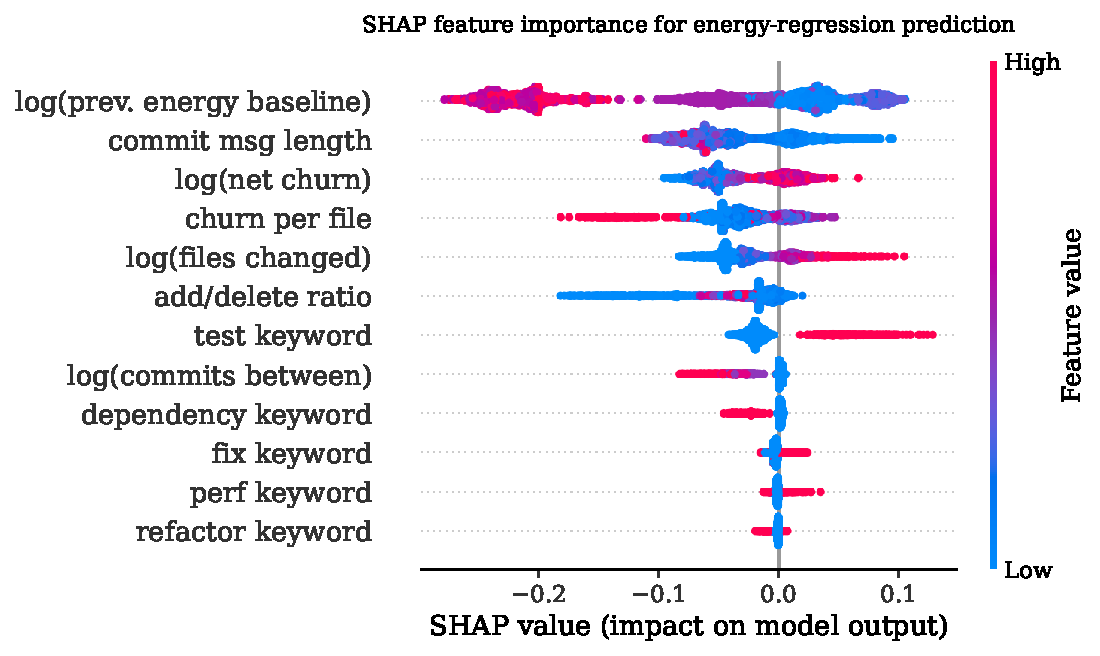
\includegraphics[width=0.75\textwidth]{figures/fig6_shap_summary.pdf}
\caption{SHAP summary plot for the final model trained on all 3{,}684 transitions.}
\label{fig:shap}
\end{figure}

\section{Discussion}
\label{sec:discussion}

Our central empirical finding is that naive cross-validation overstates the cross-project generalization of an energy-regression predictor by a statistically significant margin, and that this margin survives a threshold-sensitivity check. This mirrors, in a new task domain, findings already established in cross-project defect prediction~\citep{cpdp2026domainadaptation} and CI/CD build prediction~\citep{buildpred2026taxonomy}, and adds empirical weight to the broader argument that cross-project software prediction tasks should, by default, be evaluated with project-disjoint (or stricter) protocols rather than random splits.

A second, more nuanced finding is that project-level grouping is a necessary but not obviously sufficient safeguard on its own. The near-duplicate audit (Section~\ref{sec:dupaudit}) shows that trivial, repetitive commits are common enough (48.9\% of transitions) that near-duplicate memorization was a reasonable initial hypothesis for part of the naive-protocol inflation. However, the fold-count-matched redesign in Section~\ref{sec:redesign} isolates this cleanly: deduplicating near-identical training instances \emph{lowered} held-out performance slightly (0.488 vs. 0.545) rather than raising it, indicating near-duplicate memorization is not a meaningful contributor to the gap in this dataset. This is a useful, disconfirming result: it would have been easy to assume near-duplicate leakage was a major factor by analogy with other domains (e.g., malware detection), and our properly controlled test suggests otherwise here.

The feature ablation in Section~\ref{sec:ablation} instead identifies the previous-commit energy baseline feature (\texttt{log\_prev\_energy}) as the larger, more direct driver: removing it shrinks the naive-vs-grouped gap by roughly 62\% (0.168 to 0.064), though a smaller, still-significant gap remains. This is consistent with the mechanism we hypothesized -- the feature's project-specific absolute scale (e.g., \texttt{jsoup}'s typical readings are roughly an order of magnitude lower than \texttt{fastexcel}'s) partially lets the naive protocol infer project identity rather than learn purely diff-level signal -- but does not fully explain the gap, indicating genuine cross-project generalization difficulty beyond this one feature as well. Taken together with the algorithm-robustness check in Section~\ref{sec:algcompare}, which confirms the same direction of effect across Random Forest, XGBoost, and logistic regression via pooled bootstrap, we consider the core finding well-supported, while now understanding its two largest contributing mechanisms (feature-mediated project-identity leakage, and residual cross-project difficulty) more precisely than an unstructured "leakage exists" claim would convey.

Absolute predictive performance remains modest under the realistic (project-grouped) protocol -- ROC-AUC 0.545, only modestly above chance, and, as Section~\ref{sec:heuristic} shows plainly, not reliably better than a training-free code-churn heuristic (0.616) adapted from classic defect-prediction literature~\citep{nagappan2005churn}. We view this as an honest and reportable finding rather than a shortcoming to be hidden: it indicates that simple diff-count and keyword features are insufficient to reliably predict energy regressions across previously unseen projects, and that the specific value added by machine learning over a much simpler rule is not yet established for this task. This motivates richer, semantic features (e.g., static-analysis-derived complexity deltas, allocation and loop pattern counts) as a concrete direction for future work, discussed further in Section~\ref{sec:conclusion} -- future work in this area should demonstrate improvement over the heuristic baseline, not merely over chance. The manual verification in Section~\ref{sec:manualcheck} further complicates the interpretation of even this modest performance figure: if roughly half of the positive class consists of measurement artifacts and methodology confounds (release-metadata commits, test-suite-size growth) rather than genuine energy regressions, then the classifier's true task is muddier than ``predict energy regressions'' -- it is closer to ``predict a mixture of energy regressions, release-process commits, and test-suite growth,'' which is a less scientifically clean target. We regard this as the most consequential open issue raised by our own audit process, more so than any of the statistical robustness questions resolved above, and we discuss its implications in Section~\ref{sec:threats}.

\section{Threats to validity}
\label{sec:threats}

\textbf{Label construct validity (the most consequential open issue).} Manual verification (Section~\ref{sec:manualcheck}) of a 12-commit sample of our 52 statistically-gated regressions found only 6 (50\%) to be plausible genuine code-efficiency regressions; 3 (25\%) were release-metadata-only commits (version bumps, changelogs) with no functional code change, 1 modified only test code (mechanically inflating measured energy by running more tests, not by making production code less efficient), and 1 occurred at an early, low-baseline point in its project's history that mechanically inflates percent-change. We report this as an unresolved limitation, not a solved one: at this sample size we cannot precisely estimate the true proportion of artifact-driven labels in the full 52, and we did not re-run our evaluation with these categories filtered out. We recommend that any reuse of this benchmark first apply a filter excluding release-process and test-only commits, and we flag that our absolute predictive-performance figures should be read with this caveat in mind. Notably, this concern applies to label \emph{correctness}, not directly to the naive-vs-grouped evaluation-protocol comparison that is this paper's central claim -- that comparison holds for whatever the labels represent, artifact-influenced or not -- but it substantially qualifies what the benchmark can be said to measure.

\textbf{Single measurement source.} All energy readings originate from one data release, collected on one researcher's hardware profile using \texttt{perf}/RAPL~\citep{bechet2026energytrackr}. We cannot verify whether these measurements, or the regressions labeled from them, would replicate on different hardware, operating systems, or power governors. This is a genuine external-validity limitation that only independent replication on separate hardware can address.

\textbf{Small, imbalanced positive class.} Despite extending the benchmark to nine projects, positives remain rare (52 of 3{,}684 transitions, 1.41\%). Per-project results for projects with very few or zero positive labels (Table~\ref{tab:breakdown}) are individually unstable, which is why we report pooled, bootstrapped estimates as the primary result rather than raw per-fold numbers, and Section~\ref{sec:algcompare} shows raw fold-averaging can even reverse the apparent direction of an effect at this sample size.

\textbf{Simple feature set.} Our features are diff- and keyword-based rather than semantic (no abstract-syntax-tree-level or static-analysis-derived features). The modest absolute performance under the project-grouped protocol should be read as a property of this feature set, not necessarily of the underlying task's predictability.

\textbf{Preliminary cross-language evidence.} Only two of the nine projects are non-Java (both Go), so the cross-language dimension of our benchmark should be read as a first look rather than a robust generalization claim.

\textbf{Threshold and effect-size cutoffs.} The 20\% regression threshold and the medium-effect-size cutoff ($|\delta|>0.33$) are inherited from EnergyTrackr's default configuration and a conventional effect-size categorization~\citep{romano2006exploring}, respectively, rather than derived from this dataset. The threshold-sensitivity sweep (Section~\ref{sec:results}) partially mitigates this concern by showing the qualitative finding is stable in direction across a plausible range, though not perfectly monotonic in magnitude, and each threshold's estimate is a single-run point without its own bootstrap interval.

\textbf{Single algorithm family for the main results.} While Section~\ref{sec:algcompare} confirms the core direction of effect across three algorithms, the detailed results elsewhere in this paper (SHAP explainability, per-project breakdown, threshold sensitivity) use only Random Forest with manually fixed, untuned hyperparameters. The absolute performance figures in this paper should not be read as an upper bound on what is achievable with this feature set.

\section{Conclusion and future work}
\label{sec:conclusion}

We constructed, to our knowledge, the first cross-project, cross-language machine-learning benchmark for software energy-regression prediction, built on top of the publicly released EnergyTrackr measurements, with statistically-gated labels and a near-duplicate audit that together support three evaluation protocols of increasing rigor. Naive random-split evaluation was found to overstate predictive performance relative to a realistic, leakage-aware leave-one-project-out protocol by a statistically significant margin (bootstrap gap 0.168, 95\% CI [0.112, 0.232], $p<0.0001$), a finding that is robust to the choice of regression-labeling threshold, to a cluster-level (block-by-project) bootstrap, to a false-discovery-rate correction on the labeling procedure, and consistent in direction across three algorithm families. A feature-ablation test traced roughly 62\% of the gap's magnitude to a single project-identity-correlated feature, with a smaller residual gap remaining, and a fold-count-matched redesign of the cluster-disjoint protocol indicated near-duplicate memorization is not the dominant driver. We release the benchmark dataset, labeling code, and evaluation pipeline to support reproducible future work in this area.

Manual verification of a labeled-regression sample, however, surfaced a substantive limitation we did not anticipate at the outset: only half of the sampled labels corresponded to plausible genuine code-efficiency changes, with the remainder attributable to release-metadata commits and test-suite-size growth rather than production-code regressions. We regard resolving this construct-validity question -- through systematic filtering of release-process and test-only commits, and ideally independent manual labeling with inter-rater agreement -- as a higher near-term priority for this line of work than further algorithmic refinement, and we recommend it as the first step for anyone extending this benchmark.

Future work should pursue five directions: (1) independent replication on different hardware to test whether labeled regressions generalize beyond one measurement environment; (2) systematic filtering and re-labeling to exclude release-metadata and test-only commits, re-evaluating whether the naive-vs-grouped gap and its magnitude persist on a construct-valid subset; (3) richer, semantic code features (e.g., static-analysis-derived complexity deltas, allocation and loop pattern counts) to improve on the modest project-grouped performance observed here; (4) an anomaly-detection framing (e.g., isolation forests or one-class classifiers) as an alternative to standard supervised classification, given the persistent severe class imbalance; and (5) expansion of the cross-language dimension beyond the two Go projects studied here, ideally toward a benchmark spanning several languages in comparable proportions.

\section*{CRediT authorship contribution statement}
\textbf{Rahat Ahmed Jobu}: Conceptualization, Methodology, Software, Validation, Formal analysis, Investigation, Data curation, Writing -- original draft, Writing -- review \& editing, Visualization.

\section*{Declaration of competing interest}
The author declares that he has no known competing financial interests or personal relationships that could have appeared to influence the work reported in this paper.

\section*{Data availability}
The raw energy measurements underlying this study are publicly available from the EnergyTrackr data release (\url{https://github.com/flipflop133/energytrackr-data}). The cross-project benchmark dataset, statistical labeling code, feature-engineering pipeline, and evaluation scripts constructed in this study will be made available in a public GitHub repository upon publication; the repository is maintained privately during peer review and can be shared with editors and reviewers on request.

\section*{Acknowledgments}
The author thanks the EnergyTrackr project team for making their raw energy measurement data publicly available, which made this study possible without dedicated energy-measurement hardware.

\bibliographystyle{elsarticle-num}
\bibliography{references}

\end{document}
